% Presentation Beamer
% Characteristics:
% -- Several Themes
% -- 

%%%%%%%%%%%%%%%%%%%%%%
%%%%%%%%%%%%%%%%%%%%%%
%%% Document Start %%%
%%%%%%%%%%%%%%%%%%%%%%
%%%%%%%%%%%%%%%%%%%%%%

\documentclass{beamer}

%%%%%%%%%%%%%%%%%%%%%%%%
%%% General Settings %%%
%%%%%%%%%%%%%%%%%%%%%%%%

%%% Packages %%%
\usepackage{verbatim}
\usepackage{graphicx}
\usepackage{subfig}
\usepackage{float}
\usepackage[ruled,linesnumbered]{algorithm2e}

%%% Definitions %%%

%%% Theme Selection %%%
%\usetheme{AnnArbor}
\usetheme{Antibes}
%\usetheme{Bergen}
%\usetheme{Berkeley}
%\usetheme{Berlin}
%\usetheme{Boadilla}
%\usetheme{boxes}
%\usetheme{CambridgeUS}
%\usetheme{Copenhagen}
%\usetheme{Darmstadt}
%\usetheme{default}
%\usetheme{Frankfurt}
%\usetheme{Goettingen}
%\usetheme{Hannover}
%\usetheme{Ilmenau}
%\usetheme{JuanLesPins}
%\usetheme{Luebeck}
%\usetheme{Madrid}
%\usetheme{Malmoe}
%\usetheme{Marburg}
%\usetheme{Montpellier}
%\usetheme{PaloAlto}
%\usetheme{Pittsburgh}
%\usetheme{Rochester}
%\usetheme{Singapore}
%\usetheme{Szeged}
%\usetheme{Warsaw}

%%% PDF Subject Catalog %%%
% - This is only inserted into the PDF information catalog. Can be left
% out.
\subject{Reinforcement Learning}

%%% Institution Logo %%% - Optional
% If you have a file called "university-logo-filename.xxx", where xxx
% is a graphic format that can be processed by latex or pdflatex,
% resp., then you can add a logo as follows:
\pgfdeclareimage[height=0.5cm]{university-logo}{university-logo-filename}
\logo{\pgfuseimage{university-logo}}

%%%%%%%%%%%%%%%%%%%%%%%%%%
%%% Presentation Cover %%%
%%%%%%%%%%%%%%%%%%%%%%%%%%

%%% Presentation Title %%%
\title{Reinforcement Learning and Genetic Algorithms}

%%% Subtitle %%% - Optional
\subtitle{and Other RL Methods}

%%% Presentation Authors %%%%
% - Give the names in the same order as the appear in the paper.
% - Use the \inst{?} command only if the authors have different
%   affiliation.
\author{Rene Gutierrez$^1$, Keller Jordan$^2$}

%%% Author Affiliation %%% - Optional
% - Use the \inst command only if there are several affiliations.
% - Keep it simple, no one is interested in your street address.
\institute[University of California Santa Cruz]
{
\inst{1}%
Department of Applied Mathematics \& Statistics \\
UCSC
\and
\inst{2}%
Department of Computer Science\\
UCSC
}


%%% Conference Name and Information %%% - Optional
% - Either use conference name or its abbreviation.
% - Not really informative to the audience, more for people (including
%   yourself) who are reading the slides on-line
\date{CMPS290, Winter 2018}

%%% Table of Contents %%% - Optional
% Delete this, if you do not want the table of contents to pop up at
% the beginning of each subsection:
\begin{comment}
\AtBeginSubsection[]
{
\begin{frame}<beamer>{Outline}
\tableofcontents[currentsection,currentsubsection]
\end{frame}
}
\end{comment}

%%%%%%%%%%%%%%%%%%%%%%%%%%%%
%%% Presentation Content %%%
%%%%%%%%%%%%%%%%%%%%%%%%%%%%

\begin{document}
	
	%%% Title Page %%%
	\begin{frame}
		\titlepage
	\end{frame}
	
	
	%%% Outline %%% - Optional
	% - You might wish to add the option [pausesections]
	% - Section and subsections will appear in the presentation overview
	% and table of contents.
	%\begin{frame}{Outline}
	%  \tableofcontents
	%\end{frame}
	
	%%% Body %%%
	\graphicspath{{figures/}}
	
	\section*{Introduction}
	
	\begin{frame}{Motivation}
		\begin{block}{What we have done so far}
			\begin{itemize}
				\item Supervised Learning:
				\begin{itemize}
					\item Classification
					\item Regression
				\end{itemize}
				\item Unsupervised Learning:
				\begin{itemize}
					\item Clustering
					\item Dimensionality Reduction
					\item Density Estimation
				\end{itemize}
			\end{itemize}
		\end{block}
	\end{frame}
	
	\begin{frame}
		\begin{figure}
			\centering
			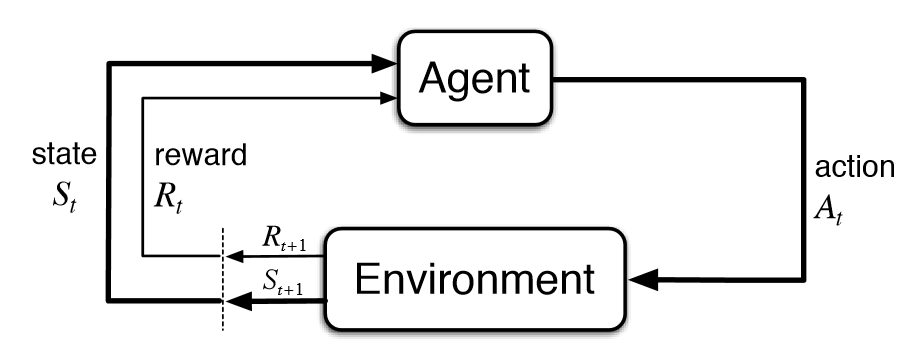
\includegraphics[width=\textwidth]{reinforcementLearning.png}
		\end{figure}
	\end{frame}
	
	\begin{frame}{Examples: Cart-Pole Problem}
		\begin{minipage}{3cm}
			\centering
			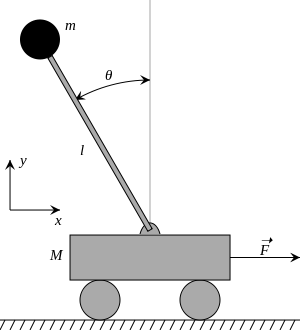
\includegraphics[width=\textwidth]{cartPole.png}
		\end{minipage}%
		\begin{minipage}{1cm}
			.
		\end{minipage}%
		\begin{minipage}{7cm}
			\textbf{Objective:} Balance a pole on top of a movable cart.
			
			\textbf{State:} Angle, angular speed, position, horizontal velocity.
			
			\textbf{Action:} Horizontal force applied to the cart $ \vec{F} $.
			
			\textbf{Reward:} 1 at each time step if the pole is upright.
		\end{minipage}
	\end{frame}
	
	\begin{frame}{Examples: Robot Locomotion}
		\begin{minipage}{3cm}
			\centering
			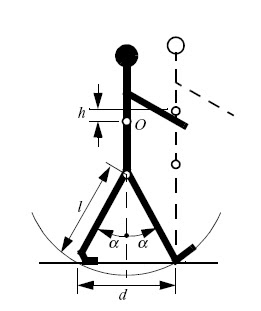
\includegraphics[width=\textwidth]{robotLocomotion.jpg}
		\end{minipage}%
		\begin{minipage}{1cm}
			.
		\end{minipage}%
		\begin{minipage}{7cm}
			\textbf{Objective:} Make a Robot move forward.
			
			\textbf{State:} Angle and Position of joints.
			
			\textbf{Action:} Torques applied to joints.
			
			\textbf{Reward:} 1 at each time step if robot moves forward and remains standing.
		\end{minipage}
	\end{frame}
	
	\begin{frame}{Examples: Atari Games}
		\begin{minipage}{3cm}
			\begin{figure}[h!]
				\centering
				\subfloat[Frostbite]{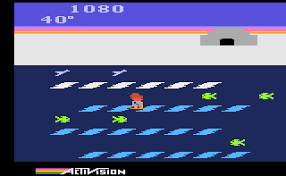
\includegraphics[width=0.8\linewidth]{frostbite.png}} \\
				\subfloat[Pong]{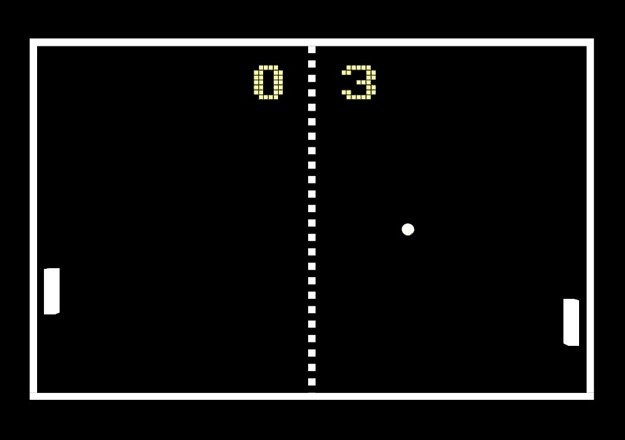
\includegraphics[width=0.8\linewidth]{pong.jpg}}                    \\
				\subfloat[Space Inv]{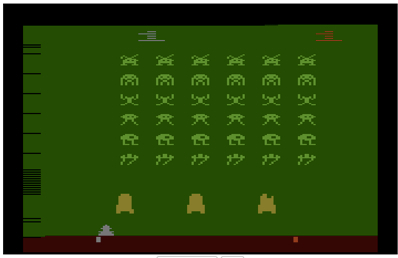
\includegraphics[width=0.8\linewidth]{spaceInvaders.jpg}} \\
			\end{figure}
		\end{minipage}%
		\begin{minipage}{1cm}
			.
		\end{minipage}%
		\begin{minipage}{7cm}
			\textbf{Objective:} Achieve the highest score.
			
			\textbf{State:} Raw pixel image of the game state.
			
			\textbf{Action:} Game controls. Usually Left, Right, Up, Down.
			
			\textbf{Reward:} Score increase or decrease at each time step.
		\end{minipage}
	\end{frame}
	
	\begin{frame}{Examples: GO}
		\begin{minipage}{3cm}
			\centering
			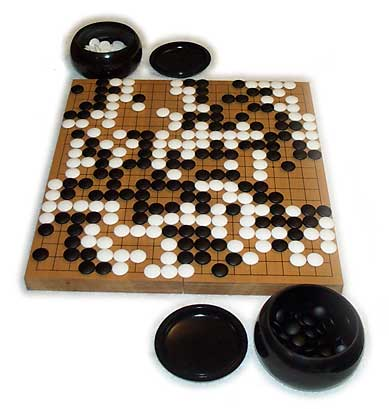
\includegraphics[width=\textwidth]{go.jpg}
		\end{minipage}%
		\begin{minipage}{1cm}
			.
		\end{minipage}%
		\begin{minipage}{7cm}
			\textbf{Objective:} Win the Game.
			
			\textbf{State:} Position of the pieces.
			
			\textbf{Action:} Next move, where to put the next piece down.
			
			\textbf{Reward:} $\begin{cases}
			1 & \text{if you win the game}   \\
			0 & \text{if you loose the game} \\
			\end{cases}$
		\end{minipage}
	\end{frame}
	
	\begin{frame}{Theoretical Background}
		\begin{block}{Reinforcement Learning}
			An Agent interacting with an environment trying to maximize a cumulative reward. The environment is typically modeled as a Markov Decision Process consisting on:
			\begin{itemize}
				\item $ \mathcal{S} $: A set of possible states.
				\item $ \mathcal{A} $: A set of possible actions.
				\item $ \mathcal{R} $: A reward distribution on states and actions.
				\item $ \mathbb{P} $: A transition probability distribution given a state and action.
				\item $ \gamma $: A discount factor.
			\end{itemize}
		\end{block}
	\end{frame}
	
	\begin{frame}{Theoretical Background}
		\begin{block}{Key Ideas}
			\begin{itemize}
				\item Markov Property: The current state completely characterises the state of the world (can be relaxed).
				\item Policy: A policy $ \pi:\mathcal{S}\to\mathcal{A} $, is mapping that assigns an action $ a \in \mathcal{A} $ to every state $ s \in \mathcal{S}$. Or $ \pi:\mathcal{S}\to f_\mathcal{A} $ if stochastic.
				\item Objective: Find a policy $ \pi^* $ such that:
				$$ \pi^* = \text{arg} \max_{\pi} \mathbb{E} \left[ \sum_{t\geq0}\gamma^t r_t  \mid \pi \right] $$
				$$ S_0 \sim \mathbb{P} \left( s_0 \right), a_t \sim \pi \left(\cdot\mid s_t\right), s_{t+1} \sim \mathbb{P}\left(\cdot \mid s_t,a_t \right) $$
			\end{itemize}
		\end{block}
	\end{frame}
	
	\begin{frame}{Theoretical Background}
		\begin{block}{Optimal Policy Example}
			\centering
			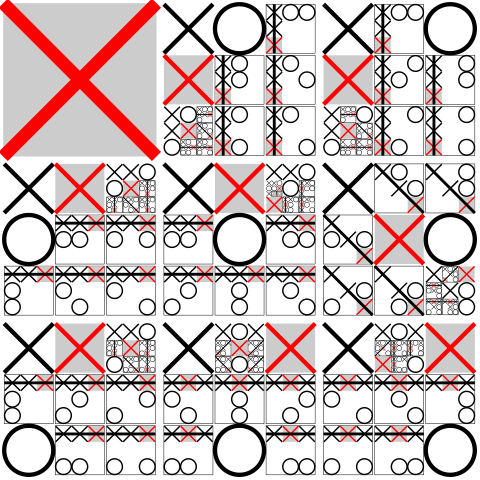
\includegraphics[width=0.4\textwidth]{TicTacToe.png}
		\end{block}
	\end{frame}
	
	\begin{frame}{Theoretical Background}
		\begin{block}{Value Function}
			The value function is a function that assigns a value to each state $ s \in \mathcal{S} $ according to the expected cumulative reward following a given policy. That is $ V^{\pi}:\mathcal{S} \to \mathbb{R} $, and is given by:
			$$ V^\pi(s) = \mathbb{E} \left[ \sum_{t\geq0}\gamma^t r_t  \mid s_0 = s,\pi \right] $$
		\end{block}
		This function tell us how good is a state.
	\end{frame}
	
	\begin{frame}{Theoretical Background}
		\begin{block}{Q-value Function}
			The Q-value function is a function that assigns a value to each pair of state $ s \in \mathcal{S} $ and action $ a \in \mathcal{A} $ according to the expected cumulative reward of taking an action and then following a given policy. That is $ Q^{\pi}:\mathcal{S}\times \mathcal{A} \to \mathbb{R} $, and is given by:
			$$ Q^\pi(s,a) = \mathbb{E} \left[ \sum_{t\geq0}\gamma^t r_t  \mid s_0 = s,a_0=a,\pi \right] $$
		\end{block}
	\end{frame}
	
	\begin{frame}{Theoretical Background}
		\begin{block}{Q-value Function}
			The Q-value function is a function that assigns a value to each pair of state $ s \in \mathcal{S} $ and action $ a \in \mathcal{A} $ according to the expected cumulative reward of taking an action and then following a given policy. That is $ Q^{\pi}:\mathcal{S}\times \mathcal{A} \to \mathbb{R} $, and is given by:
			$$ Q^\pi(s,a) = \mathbb{E} \left[ \sum_{t\geq0}\gamma^t r_t  \mid s_0 = s,a_0=a,\pi \right] $$
		\end{block}
	\end{frame}
	
	\begin{frame}{Theoretical Background}
		\begin{block}{Optimal Q-value function}
			The optimal Q-value function is a function that maximizes the expected cumulative reward achievable at each pair of state $ s \in \mathcal{S} $ and action $ a \in \mathcal{A} $. That is $ Q^*:\mathcal{S}\times \mathcal{A} \to \mathbb{R} $, and is given by:
			$$ Q^*(s,a) = \max_\pi \mathbb{E} \left[ \sum_{t\geq0}\gamma^t r_t  \mid s_0 = s,a_0=a,\pi \right] $$
		\end{block}
	\end{frame}
	
	\begin{frame}{Theoretical Background}
		\begin{block}{Bellman Equation}
			Principle of Optimality: An optimal policy has the property that whatever the initial state and initial decision are, the remaining decisions must constitute an optimal policy with regard to the state resulting from the first decision. (See Bellman, 1957, Chap. III.3.)
			$$ Q^*(s_t,a_t) = \mathbb{E}_{s_{t+1}} \left[ r_t + \gamma \max_{a_{t+1}} Q^*(s_{t+1},a_{t+1})  \mid s_t,a_t \right] $$
		\end{block}
	\end{frame}
	
	\begin{frame}{Theoretical Background}
		\begin{block}{Value Iteration}
			We cn use the Bellman Equation as an iterative update
			$$ Q_{i+1}(s_t,a_t) = \mathbb{E}_{s_{t+1}} \left[ r_t + \gamma \max_{a_{t+1}} Q_{i}(s_{t+1},a_{t+1})  \mid s_t,a_t \right] $$
			where we will have that:
			$$ Q_i \to Q^* \text{as} i \to \infty $$
		\end{block}
	\end{frame}
	
	\section*{Infinite State Spaces}
	
	\begin{frame}{Problem: What do we do in continuous state spaces?}
		\begin{itemize}
			\item Frame-based games (Atari)
			\item Robotics control tasks
		\end{itemize}
	\end{frame}
	
	\begin{frame}{Solution: use an approximation to $Q(s, a)$ or $\pi(a | s)$}
		\begin{figure}
			\centering
			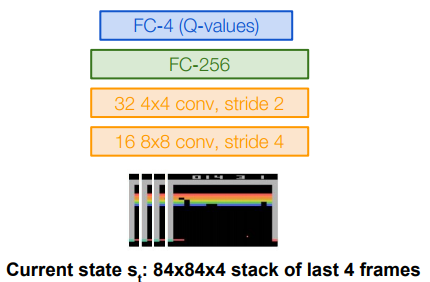
\includegraphics[height=0.7\textheight]{dqn_architecture.png}
		\end{figure}
	\end{frame}
	
	\begin{frame}{How can we train deep Q-Networks or Policy-Networks?}
		\begin{itemize}
			\item Deep Q-Learning
			\item A3C
			\item Evolution Strategies (ES)
			\item Genetic Algorithms (GA)
		\end{itemize}
	\end{frame}
	
	\section*{Training Methods}
	
	\subsection*{Deep Q-Learning}
	
	\begin{frame}
		\Huge Deep Q-Learning
		\footnote{Mnih, V., Kavukcuoglu, K., Silver, D., Graves, A., Antonoglou, I., Wierstra, D., and Riedmiller, M.
(Dec 2013). Playing Atari with deep reinforcement learning. Technical Report arXiv:1312.5602
[cs.LG], Deepmind Technologies.}
	\end{frame}
	
	\begin{frame}{Key Features}
		\begin{itemize}
			\item Variant of Q-Learning where we use gradient descent to update model parameters
			\item Uses ``replay memory" containing last $N$ experienced transitions, from which minibatches are drawn. This increases data efficiency and decreases variance of updates.
			\item Surpassed human performance on 3/7 games
		\end{itemize}
	\end{frame}
	
	\begin{frame}{Algorithm}
		\begin{figure}
			\centering
			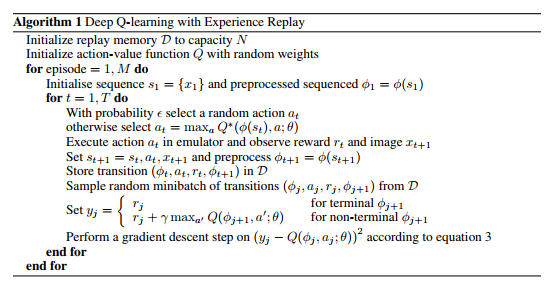
\includegraphics[height=0.7\textheight]{dqn_algorithm.png}
		\end{figure}
	\end{frame}
	
	\begin{frame}{Results}
		\begin{figure}
			\centering
			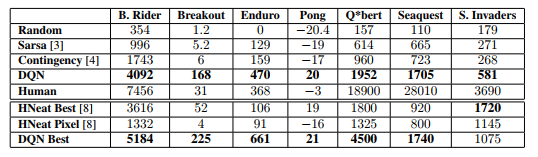
\includegraphics[width=1.2\textheight]{dqn_results.png}
		\end{figure}
	\end{frame}
	
	
	\subsection*{Policy Gradients}
	
	\begin{frame}
		\begin{block}{Key Ideas}
			We can explore a parametrized space of the policy functions:
			$$ \Pi = \{ \pi_\theta \mid \theta \in \mathbb{R}^m \} $$
			and define the corresponding cumulative expected reward
			$$ J(\theta) = \mathbb{E} \left[ \sum_{t\geq0}\gamma^t r_t  \mid \pi_\theta \right] $$
			and solve
			$$ \theta^* = \text{arg} \max_\theta J(\theta) $$
		\end{block}
	\end{frame}
	
	\begin{frame}
		\begin{block}{Key Ideas}
			If we define a trajectory $ \tau $ as:
			$$ \tau = \left( s_0,a_0,r_0,s_1,\ldots \right) $$
			and the reward associated with it as:
			$$ r(\tau) $$
			we have that:
			$$ J(\theta) = \mathbb{E}_{\tau \sim \mathbb{P}(\tau ; \theta) } \left[ r(\tau) \right] $$
		\end{block}
	\end{frame}
	
	\begin{frame}
		\begin{block}{Key Ideas}
			How to optimize? Using gradient ascent!
			\begin{align*}
			J(\theta) &= \mathbb{E}_{\tau \sim \mathbb{P}(\tau ; \theta) } \left[ r(\tau) \right]\\
			&= \int_{\tau} r(\tau) \mathbb{P}(\tau ; \theta) d\tau \\
			\end{align*}
			And we can differentiate:
			$$ \nabla_\theta J(\theta) = \int_{\tau} r(\tau) \nabla_\theta \mathbb{P}(\tau ; \theta) d\tau $$
			which is actually hard to compute!
		\end{block}
	\end{frame}
	
	\begin{frame}
		\begin{block}{First Trick}
			\begin{align*}
			\nabla_\theta \mathbb{P}(\tau ; \theta) &= \mathbb{P}(\tau ; \theta) \frac{\nabla_\theta \mathbb{P}(\tau ; \theta)}{\mathbb{P}(\tau ; \theta)} \\
			&= \mathbb{P}(\tau ; \theta) \nabla_\theta \log \left( \mathbb{P}(\tau ; \theta) \right)
			\end{align*}
			then
			\begin{align*}
			\nabla_\theta J(\theta) &= \int_{\tau} r(\tau) \mathbb{P}(\tau ; \theta) \nabla_\theta \log \left( \mathbb{P}(\tau ; \theta) \right) d\tau \\
			&= \mathbb{E}_{\tau \sim \mathbb{P}(\tau ; \theta) } \left[ r(\tau) \nabla_\theta \log \left( \mathbb{P}(\tau ; \theta) \right) \right]
			\end{align*}
			which we can estimate using Monte Carlo sampling.
		\end{block}
	\end{frame}
	
	\begin{frame}
		\begin{block}{Second Trick}
			Note that:
			$$ \mathbb{P}(\tau ; \theta) = \prod_{t\geq0} \mathbb{P}(s_{t+1} \mid s_t, a_t) \pi_\theta (a_t \mid s_t) $$
			Then:
			$$ \log \left( \mathbb{P}(\tau ; \theta) \right) = \sum_{t\geq0} \left[  \log \left( \mathbb{P}(s_{t+1} \mid s_t, a_t) \right) + \log \left( \pi_\theta (a_t \mid s_t) \right) \right] $$
			Then:
			$$ \nabla_\theta \log \left( \mathbb{P}(\tau ; \theta) \right) = \sum_{t\geq0} \nabla_\theta \log \left( \pi_\theta (a_t \mid s_t) \right) $$
			which does not depend on the transition probabilities.
		\end{block}
	\end{frame}
	
	\begin{frame}
		\begin{block}{Result}
			Applying both tricks we have that:
			$$ \nabla_\theta J(\theta) \approx \sum_{t\geq0} r(\tau) \nabla_\theta \log \left( \pi_\theta (a_t \mid s_t) \right) $$
			Unfortunately, this estimate suffers for high variance, and a lot for trajectories would be needed to obtain a good estimate.
		\end{block}
	\end{frame}
	
	\begin{frame}
		\begin{block}{Tricks for Variance Reduction}
			\begin{itemize}
				\item Only consider future rewards. At time $ t$ instead of $ r(\tau) $ use $ \sum_{t'\geq t} r_{t'} $.
				\item Use a discount factor. That is, instead of $ \sum_{t'\geq t} r_{t'} $ use $ \sum_{t'\geq t} \gamma^{t'-t} r_{t'} $.
				\item Don't use the raw value of the reward but consider it against a base line. That is, instead of $ \sum_{t'\geq t} \gamma^{t'-t} r_{t'} $ use $ \sum_{t'\geq t} \gamma^{t'-t} r_{t'} -b(s_t) $.
				\item A good excess reward indicator is given by the Q-function and the value function. That is:
				$$ \sum_{t'\geq t} \gamma^{t'-t} r_{t'} -b(s_t) \approx Q^{\pi_\theta}(s_t,a_t) - V^{\pi_\theta} (s_t) $$
			\end{itemize}
		\end{block}
	\end{frame}
	
	\begin{frame}
		\begin{block}{Tricks for Variance Reduction}
			So to reduce the variance, use:
			$$ \nabla_\theta J(\theta) \approx \sum_{t\geq0} \left( Q^{\pi_\theta}(s_t,a_t) - V^{\pi_\theta} (s_t) \right) \nabla_\theta \log \left( \pi_\theta (a_t \mid s_t) \right) $$
			since we don't know $ Q $ and $ V $ we can use Q-learning!
		\end{block}
	\end{frame}
	
	\begin{frame}{Actor-Critic Policy Gradient Methods }
		\begin{block}{Key Ideas}
			\begin{itemize}
				\item The Actor decides the policy $ \pi_\theta $.
				\item The Critic tells the actor how good the policy is: 
				$$ A^\pi (s,a) = Q^{\pi_\theta}(s_t,a_t) - V^{\pi_\theta} (s_t) \approx \sum_{t'\geq t} \gamma^{t'-t} r_{t'} - V^{\pi_\theta} (s_t) $$
				which we can call the advantage of policy $ \pi $.
				\item The Critic only needs to learn the advantage for the policy trajectory.
			\end{itemize}
		\end{block}
	\end{frame}
	
	\begin{frame}{Actor-Critic Algorithm }
		\centering
		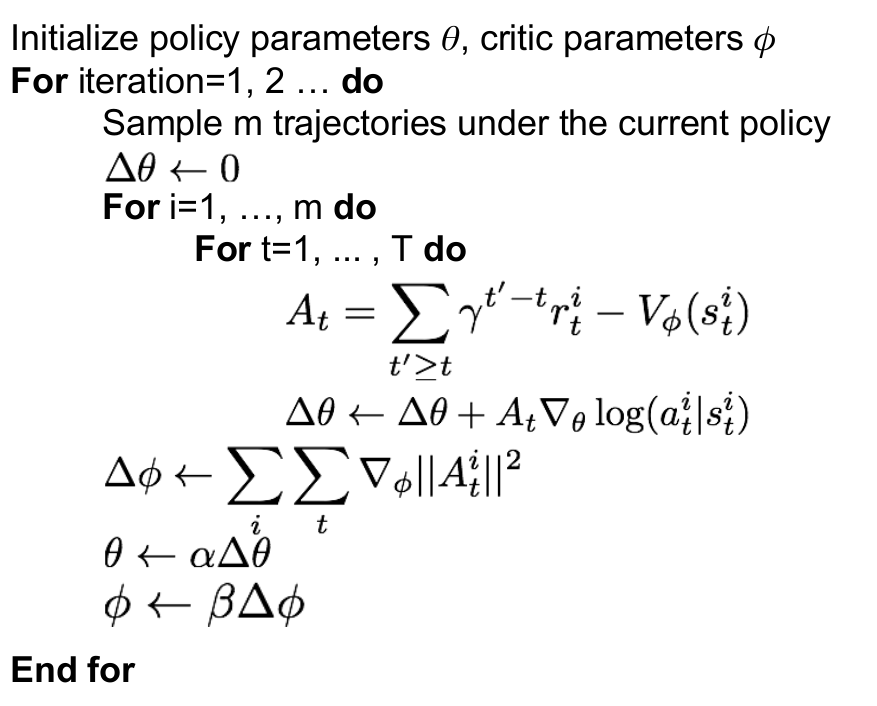
\includegraphics[height=0.8\textheight]{vanillaActorCritic.png}
	\end{frame}
	
	\begin{frame}{A3C}
		\centering
		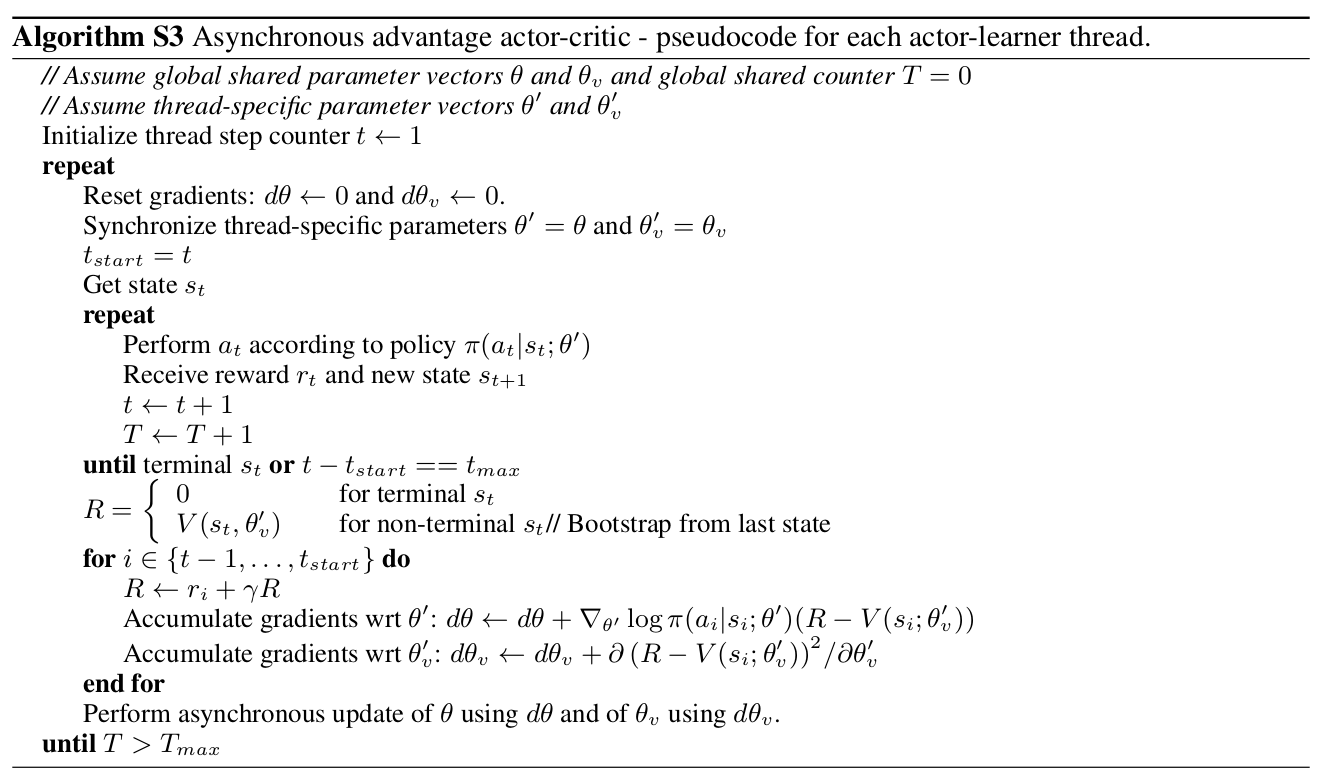
\includegraphics[height=0.8\textheight]{a3c.png}
	\end{frame}
	
	\begin{frame}{A3C Comparison}
		\centering
		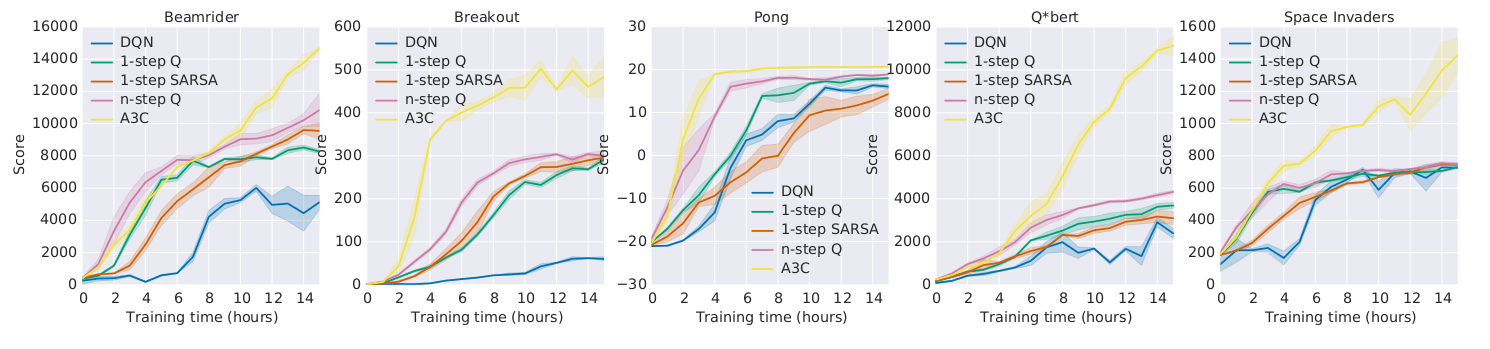
\includegraphics[width=\textwidth]{a3cScores.png}
	\end{frame}
	
	\subsection*{Evolution Strategies}
	
	\begin{frame}
		\Huge Evolution Strategies
		\footnote{Tim Salimans, Jonathan Ho, Xi Chen, and Ilya Sutskever. Evolution strategies as a scalable alternative to
reinforcement learning. arXiv preprint arXiv:1703.03864, 2017. URL http://arxiv.org/abs/1703.
03864.}
	\end{frame}
	
	\begin{frame}{Key Features}
		\begin{itemize}
			\item Simpler and fewer assumptions compared to current RL algorithms
			\item Finite-differences gradient approximation
			\item Highly parallelizable
			\item Competitive with other methods on benchmarks
		\end{itemize}
	\end{frame}
	
	\begin{frame}{Algorithm}
		\begin{figure}
			\centering
			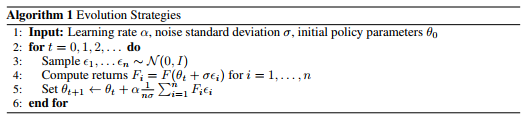
\includegraphics[width=1.2\textheight]{es_algorithm.png}
		\end{figure}
	\end{frame}
	
	\begin{frame}{Algorithm}
		\begin{figure}
			\centering
			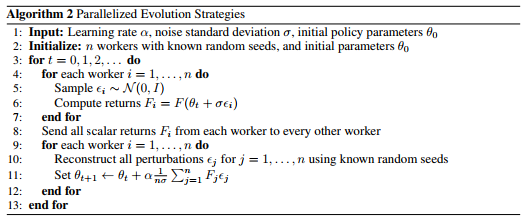
\includegraphics[width=1.2\textheight]{es_parallel.png}
		\end{figure}
	\end{frame}
	
	\begin{frame}{Results}
		\begin{itemize}
			\item On Atari, ES is competitive with A3C (does better in 23 / 51 games)
			\item Avoids complexity of Deep Q-Learning/A3C
			\begin{itemize}
				\item No backward pass or gradient updates
				\item Policy function approximator can be nondifferentiable
				\item No need to store replay memory
			\end{itemize}
			\item Highly Parallelizable (communicate only rewards if seeds are known)
			\item Therefore much lower training time when distributed across many cpus
			\item Avoids issue of credit assignment over long time scale
		\end{itemize}
	\end{frame}
	
	\subsection*{Genetic Algorithm}

	\begin{frame}
		\Huge Deep Genetic Algorithms
		\footnote{Petroski Such, Felipe, Madhavan, Vashisht, Conti,
Edoardo, Lehman, Joel, Stanley, Kenneth O., and Clune,
Jeff. Deep neuroevolution: Genetic algorithms are a
competitive alternative for training deep neural networks
for reinforcement learning. arXiv preprint to appear,
2017.}
	\end{frame}
	
	\begin{frame}{Key Features}
		\begin{itemize}
			\item Truly gradient-free method
			\item Maintains ``generation" of models, allowing for greater diversity in policies
			\item Even more parallelizable
		\end{itemize}
	\end{frame}
	
	\begin{frame}{Algorithm}
		\begin{figure}
			\centering
			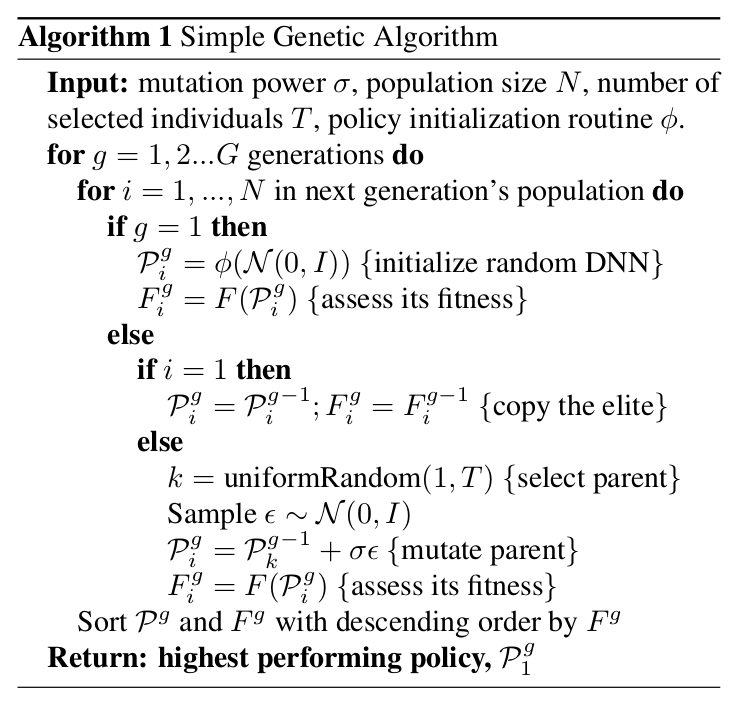
\includegraphics[height=0.7\textheight]{deep_ga_algorithm.png}
			\label{fig4}
		\end{figure}
	\end{frame}
	
	\begin{frame}{Algorithm}
		Even more parallelizable than ES
		\begin{itemize}
			\item Represent each model by the sequence of random seeds that generated it
		\end{itemize}
	\end{frame}
	
	\begin{frame}{Results}
		\begin{itemize}
			\item DQN, ES, GA all score highest on 3 games, A3C 4
			\item Sometimes GA beats other methods within first generation -- what if we try random search?
		\end{itemize}
	\end{frame}
	
	\begin{frame}{Results}
		\begin{figure}
			\centering
			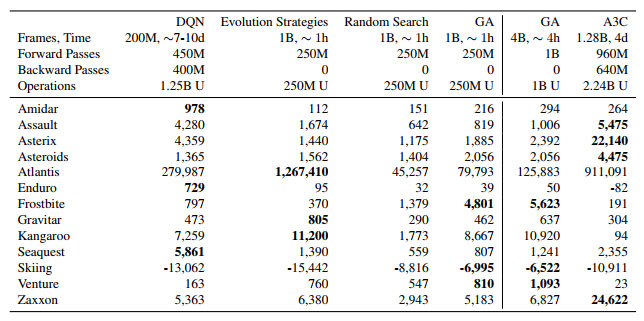
\includegraphics[width=1.2\textheight]{deep_ga_results.png}
			\label{fig4}
		\end{figure}
	\end{frame}
	
	\begin{frame}{Results}
		\begin{itemize}
			\item DQN, ES, GA all score highest on 3 games, A3C 4
			\item Sometimes GA beats other methods within first generation -- what if we try random search?
			\item Random search outperforms DQN on 4 out of 13 games, ES on 3, A3C on 5 (!)
			\item Can use novelty search techniques to solve problems no other approach can tackle
		\end{itemize}
	\end{frame}
	
	\begin{frame}{Results}
		Image Hard Maze
		\begin{figure}
			\centering
			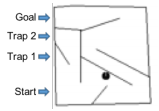
\includegraphics[width=.5\textheight]{image_hard_maze.png}
			\label{fig4}
		\end{figure}
	\end{frame}
	
	\begin{frame}
		\begin{figure}
			\centering
			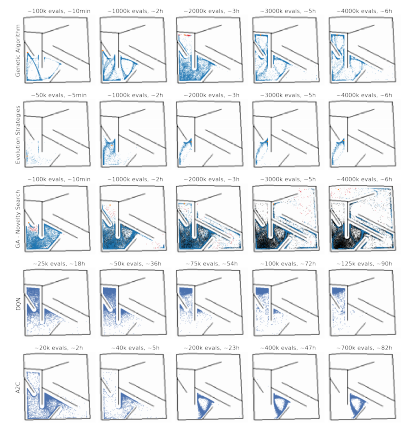
\includegraphics[width=.9\textheight]{ga_novelty.png}
			\label{fig4}
		\end{figure}
	\end{frame}
	
	\begin{frame}{Results}
		\begin{itemize}
			\item DQN, ES, GA all score highest on 3 games, A3C 4
			\item Sometimes GA beats other methods within first generation -- what if we try random search?
			\item Random search outperforms DQN on 4 out of 13 games, ES on 3, A3C on 5 (!)
			\item Can use novelty search techniques to solve problems no other approach can tackle
			\item Compact network encoding
			\begin{itemize}
				\item Number of generations is typically low for these problems (~10-200)
				\item Networks are represented as sequence of seeds to generate perturbations from initial weights
				\item 4m parameters $\rightarrow$ thousands of bytes (10,000 fold compression)
			\end{itemize}
		\end{itemize}
	\end{frame}
	
	\section*{Takeaways}
	
	\begin{frame}{Takeaways}
		\begin{itemize}
			\item Each approach performs well on some tasks and poorly on others
			\item Some standard benchmarks are simple enough to solve using random search
			\item Future research directions:
			\begin{itemize}
				\item Implement existing methods from GA literature to deep GA
				\item Potential to use nondifferentiable models (binary networks)
				\item Create new algorithms that combine best of each
			\end{itemize}
		\end{itemize}
	\end{frame}
	
	
	% All of the following is optional and typically not needed.
	\begin{comment}
	\appendix
	\section<presentation>*{\appendixname}
	\subsection<presentation>*{For Further Reading}
	
	\begin{frame}[allowframebreaks]
	\frametitle<presentation>{For Further Reading}
	
	\begin{thebibliography}{10}
	
	\beamertemplatebookbibitems
	% Start with overview books.
	
	\bibitem{Author1990}
	A.~Author.
	\newblock {\em Handbook of Everything}.
	\newblock Some Press, 1990.
	
	
	\beamertemplatearticlebibitems
	% Followed by interesting articles. Keep the list short. 
	
	\bibitem{Someone2000}
	S.~Someone.
	\newblock On this and that.
	\newblock {\em Journal of This and That}, 2(1):50--100,
	2000.
	\end{thebibliography}
	
	\end{frame}
	
	\begin{itemize}
	\item
	Outlook
	\begin{itemize}
	\item
	Something you haven't solved.
	\item
	Something else you haven't solved.
	\end{itemize}
	\end{itemize}
	
	\end{comment}
	
\end{document}